\documentclass[a4paper,fleqn,twocolumn]{ctexart}
\usepackage{geometry,graphicx,tikz}
\geometry{left=2.0cm,right=2.0cm,top=2.5cm,bottom=2.5cm}
\usepackage{amsmath}
\usepackage{amssymb}
\usepackage{graphicx}
\newcommand{\di}[1]{\mathrm{d}#1}
\newcommand{\p}[2]{\frac{\partial #1}{\partial #2}}
\newcommand{\pp}[2]{\frac{\partial ^2 #1}{\partial #2 ^2}}
\newcommand{\dy}[2]{\frac{\di{#1}}{\di{#2}}}
\newcommand{\ddy}[2]{\frac{\mathrm{d} ^2 #1}{\mathrm{d} #2 ^2}}
\newcommand{\zbj}[4]
{
\draw (0,0) node[below left] {$ O $};
\draw [->] (#1,0) -- (#2,0) node[right] {$ x $};
\draw [->] (0,#3) -- (0,#4) node[right] {$ y $};
}

\begin{document}
	\noindent\textbf{\Large 说明:}笔者并不建议按照转动定理等名称记忆刚体运动的公式。实际上这些公式都是质点运动学各定律的延伸(如角动量对应动量,转动惯量对应质量,转动定理和动量矩定理对应牛顿第二定律等),做题的时候只需要认定该问题需要用质点运动学的哪些定律,再将质量,力等物理量换成刚体运动学中的转动惯量,力矩等即可。但为了与课本表述一致,在本解析中仍然按照刚体运动学公式名称引用,但会在其后附注数学表达式以方便对应。
	\begin{section}{选择题}
		\[1.C\]\par
		直观地理解,两个系统所受合外力均为$ Mg $,图A要驱动滑轮和重物(他们都获得了加速度),图B只需要驱动滑轮,因此$ \beta_A<\beta_B $。驱动滑轮的力为$ T_A $和$ T_B $,因此必有$ T_A<T_B $。\par
		从定量计算来看,显然$ T_B=F=Mg $。对A滑轮,对物体应用牛顿第二定律$F=ma$,对滑轮应用转动定律$M=J\beta$:
		\[Mg-T_A=Ma\]
		\[T_A\times R=J\beta\]
		与$ a=\beta R $联立解得:
		\[T_A=\frac{Mg}{\frac{MR^2}{J}+1}\]
		则有$ T_A< Mg=T_B$
		\[2.D\]\par
		%此处需要配一个图来说明\theta,与竖直方向的夹角,从\pi/2到0
		\begin{tikzpicture}
			\draw[dashed](0,0) -- (3,0);
			\draw[dashed](0,0) -- (0,-3);
			\draw[dashed](3,0) arc (0:-90:3);
			\draw(0,0) -- (2.4,-1.8);
			\draw(0.5,0) arc (0:-36.87:0.5) node[right=5pt] {$ \theta $};
		\end{tikzpicture}\par
		首先此题讨论的是细棒对于$ O $点的转动惯量。由于细棒对于其一个端点的转动惯量恒为$ \frac{1}{3}ml^2 $,因此转动惯量不变。至于角加速度$ \beta $,由转动定律$M=J\beta$:
			\[Mg\frac{l}{2}\sin\theta=\frac{1}{3}ml^2\times\beta\]\par
		解得:$ \beta=\frac{3Mg\sin\theta}{2ml} $,可知$ \beta $随下落过程中$ \theta $的减少而减少,因此角加速度从大到小。
		\[3.D\]\par
		本题默认水平圆盘放在桌子上,力矩均指对轴的力矩。在玻璃球自由滚动的时候,系统受三个力:重力,支持力(与重力抵消,合力矩为0),还受轴对圆盘的支持力,但由于该力的$ \vec{r}=0 $,因此该力力矩也为0,合外力矩也为0。由动量矩定理$ M=\dy{L}{t} $知,此系统角动量守恒,D正确。若小球处于滚动状态,则轴对圆盘可能会有支持力的作用,由冲量定理$ (I=\Delta p) $,动量不守恒,A,B均错误。若小球与轴或者盘边缘碰撞,由于题目中未说明小球与轴或盘边缘的碰撞是否是完全弹性碰撞,因此碰撞可能会产生机械能损失,C错误。\\
		\textbf{\Large 注:}笔者希望同学们对这类圆盘(或细棒)受到固定轴约束转动的问题有更多了解。轴对圆盘的力有且仅有两个,分别是摩擦力和支持力。对于支持力,其垂直于作用面,因此总是指向轴心,$ \vec{r}=0 $,该力对转轴的力矩为0。至于摩擦力,由于其与相对转动速度相反,因此该力与轴相切,由于轴是有半径的(不是一条线),因此$ \vec{r}=R $(R为转轴的半径,显然摩擦力的力矩不为0(但在碰撞过程中,由于$ \Delta t\to 0 $,由动量矩定理,该力矩导致的角动量变化$ \Delta L\to 0 $,因此也可认为角动量守恒)。该题中已经说明忽略轴的摩擦,因此圆盘和小球受到的合外力矩为0。更多相关内容请参考《力学(物理类)》(舒幼生著)。
		\[4.C\]\par
		角动量的定义为$ L=\vec{r}\times m\vec{v} $,$ m $为质点质量,$ \vec{v} $为质点速度(运动状态),$ \vec{r} $为质点的向径(与坐标原点有关),C正确,ABD均错误。
		\[5.D\]\par
		%此处插一张图
		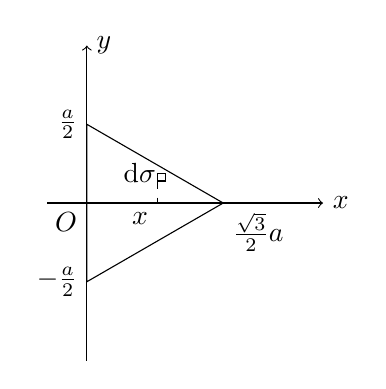
\begin{tikzpicture}
			\zbj{-0.5}{3}{-2}{2}
			\draw (0,-1) node[left] {$ -\frac{a}{2} $}
			-- (0,1) node[left] {$ \frac{a}{2} $}
			-- (1.732,0) node[below right] {$ \frac{\sqrt{3}}{2}a $}
			 -- cycle;
			\draw [dashed](0.9,0.28) -- (0.9,0);
			\node[dashed,below left] at (0.9,0) {$ x $};
			\draw (0.9,0.280) rectangle (1,0.38) node [left]{$\di{\sigma}$};
		\end{tikzpicture}\par
		微元$ \di{\sigma} $到轴的距离为$ x $。由于积分域关于$ x $轴对称,被积函数关于$ y $为偶函数,因此$ J=2J_1 $,$ J_1 $为第一象限部分的转动惯量。
		\begin{align*}
			J&=2\iint\limits_{\sigma_1}\left(m\frac{\di{\sigma}}{\frac{\sqrt{3}}{4}a^2}\right)x^2\\
			&=\frac{8m}{\sqrt{3}a^2}\int_0^{\frac{\sqrt{3}}{2}a}\di{x}\int_0^{\frac{1}{2}a-\frac{\sqrt{3}}{3}x}x^2\di{y}
			%&=\frac{8m}{\sqrt{3}a^2}\int_0^{\frac{\sqrt{3}}{2}a}\di{x}\left(\frac{1}{2}ax^2-\frac{\sqrt{3}}{3}x^3\right)\\
			%&=\frac{8m}{\sqrt{3}a^2}\left(\frac{1}{6}ax^3-\frac{\sqrt{3}}{12}x^4\right)\left.\right|_0^{\frac{\sqrt{3}}{2}a}\\
			%&=\frac{8m}{\sqrt{3}a^2}\left(\frac{\sqrt{3}}{16}a^4-\frac{3\sqrt{3}}{64}a^4\right)\\
			%&=\frac{8m}{\sqrt{3}a^2}\frac{\sqrt{3}}{64}a^4\\
			%&=\frac{1}{8}ma^2
		\end{align*}\par
		解得:$ J=\frac{1}{8}ma^2 $
		\[6.A\]\par
		直观上理解,$ \sigma(\theta) $在$ \theta=\frac{\pi}{2} $时最大,在$ \theta=0 $或$ \theta=\pi $时最小,此即球面质量更多地分布在赤道附近,两极附近质量面密度小。由于赤道附近距离$ z $轴距离更大,因此分布不均匀的球面转动惯量更大,A正确。\par
		通过计算也可以得到相同的结论,此处不再赘述。
		\[7.A\]\par
		碰撞过程中$ \Delta t\to 0 $,小球和系杆组成的系统受到4个力:重力,支持力(与重力相互抵消),O点对杆的支持力,O点对杆的摩擦力。因此系统角动量守恒(详细分析可见选择题3的“注”部分),有:
		\[0+rmv=(\frac{1}{12}ml^2+m\left(\frac{l}{2}\right))^2\omega\]
		解得:$\omega=\frac{3v}{2l}$
		\[8.C\]\par
		%此处少一张图
		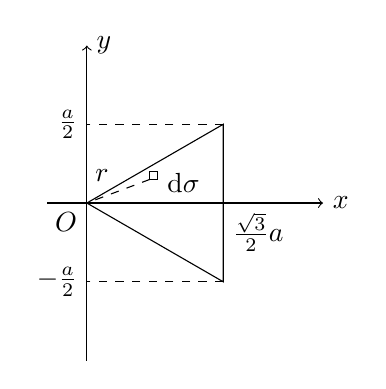
\begin{tikzpicture}
		\zbj{-0.5}{3}{-2}{2}
		\draw (0,0)-- (1.732,1) -- (1.732,-1) -- cycle;
		\draw[dashed] (1.732,1) -- (0,1) node[left] {$ \frac{a}{2} $};
		\draw[dashed] (1.732,-1) -- (0,-1) node[left] {$ -\frac{a}{2} $};
		\node[below right] at (1.732,0) {$\frac{\sqrt{3}}{2}a$};
		\draw (0.8,0.3) rectangle (0.9,0.4);
		\draw [dashed](0.8,0.3) -- node[above left] {$ r $} (0,0);
		\node [below right] at (0.9,0.5) {$\di{\sigma}$};
		\end{tikzpicture}\par
		微元$ \di{\sigma} $到轴(就是到原点)的距离为$ \sqrt{x^2+y^2} $。由于积分域关于$ x $轴对称,被积函数关于$ y $为偶函数,因此$ J=2J_1 $,$ J_1 $为第一象限部分的转动惯量。
		\begin{align*}
		J&=2\iint\limits_{\sigma_1}\left(m\frac{\di{\sigma}}{\frac{\sqrt{3}}{4}a^2}\right)(x^2+y^2)\\
		&=\frac{8m}{\sqrt{3}a^2}\int_0^{\frac{\sqrt{3}}{2}a}\di{x}\int_0^{\frac{\sqrt{3}}{3}x}(x^2+y^2)\di{y}
		\end{align*}\par
		解得:$ J=\frac{5}{12}ma^2 $
		\[9.A\]\par
		由动量矩定理易知A正确。BCD均为充分条件。小球在绳子的束缚下绕定点做匀速圆周运动,则所受合外力不为0(绳子的拉力),B错误,且小球受到的重力和支持力对定点的力矩均不为0,因此受到了外力矩的作用,C错误。对于D,可令$ J=t,\omega=\frac{1}{t} $,则$ L=J\omega=1 $,角动量守恒,但转动惯量和角速度都在随时间变化,因此D错误。
		\[10.A\]\par
		卫星做匀速圆周运动,则$ m,v,r $均不变,$ \vec{r}\times\vec{v} $的方向也不变,因此角动量守恒。卫星与地球的万有引力与卫星的运动方向恒垂直,因此卫星与地球构成的系统的内力(万有引力)不做功,同时又不受外力作用,因此卫星的动能守恒。
	\end{section}

	\begin{section}{填空题}
		\[11.\frac{3M}{ma} \hspace{2em} \frac{18M^2}{m^2a^3}t^2\]\par
		本题中转动方向固定,用标量形式计算即可。
		\begin{gather*}
			\beta=\frac{M}{J}=\frac{6M}{ma^2}\\
			\text{开始时}\omega=0,\quad\therefore \omega=\frac{6M}{ma^2}t\\
			v=\omega r=\frac{6M}{ma^2}t\times\frac{a}{2}=\frac{3M}{ma}t\\
			\alpha_{\tau}=\dy{v}{t}=\frac{3M}{ma}\\
			\alpha_n=\frac{v^2}{r}=\frac{\left(\frac{3M}{ma}t\right)^2}{\frac{a}{2}}=\frac{18M^2}{m^2a^3}t^2
		\end{gather*}
		\[12.\frac{1}{12}mR^2\omega_0^2\]\par
		圆柱所受合外力为摩擦力$f$,效果使得圆柱的质心运动速度$ v_c $增大。\par
		圆柱所受合外力矩为摩擦力矩$ M_f $,效果使得圆柱的角速度$ \omega $减小。\par
		圆柱做纯滚动的瞬间,即$ v_c=\omega R $。因此求得$ v_c $和$ \omega $对时间的函数,解出$ t $即可。\par
		对圆柱使用牛顿第二定律$F=ma$和转动定律$M=J\beta$:
		\begin{gather*}
			a_c=\frac{f}{m}=\mu g\quad\therefore v_c=0+\mu gt=\mu gt\\
			\beta=\frac{M}{J}=\frac{-\mu mgR}{\frac{1}{2}mR^2}=-\frac{2\mu g}{R}\\
			\therefore \omega=\omega_0+\beta t=\omega_0-\frac{2\mu g}{R}t\\
			\text{代入纯滚关系式:}\mu gt=\omega_0R-2\mu gt\\
			\therefore t=\frac{\omega_0R}{3\mu g}\\
			\text{此时}v_c=\mu g\frac{\omega_0R}{3\mu g}=\frac{\omega_0R}{3}\\
			\hspace{2em}\omega=\omega_0-\frac{2\mu g}{R}\frac{\omega_0R}{3\mu g}=\frac{\omega_0}{3}
		\end{gather*}\par
		由柯尼希定理:
		\begin{align*}
			E_{\text{总}}&=\frac{1}{2}mv_c^2+\frac{1}{2}J\omega^2\\
						&=\frac{1}{2}m\left(\frac{\omega_0R}{3}\right)^2+\frac{1}{2}\left(\frac{1}{2}mR^2\right)\left(\frac{\omega_0}{3}\right)^2\\
						&=\frac{1}{12}mR^2\omega_0^2
		\end{align*}
		\[14.\frac{1}{8}Mg\]
		物体加速度$ a $与滑轮角加速度$ \beta $的关系为:
		\[\beta=\frac{a}{R}=\frac{g}{4R}\]
		对滑轮应用转动定律$M=J\beta$:
		\begin{gather*}
			TR=\frac{1}{2}MR^2\beta\\
			\therefore T=\frac{MR^2}{2R}\frac{g}{4R}=\frac{1}{8}Mg
		\end{gather*}
		\[15.\frac{1}{2l}\left(\sqrt{\frac{3gl}{2}}+\frac{v_0}{2}\right)\]\par
		首先计算碰撞前杆的角速度,由机械能守恒:
		\begin{gather*}
			0+0=Mg(-\frac{l}{2}\sin 30^\circ)+\frac{1}{2}J\omega^2\\
			\omega_1=\sqrt{\frac{Mgl}{4}\frac{2}{\frac{1}{3}Ml^2}}=\sqrt{\frac{3g}{2l}}
		\end{gather*}\par
		以杆和子弹为系统,在碰撞过程中,所受外力里只有O点对杆的支持力为无穷大(抵消子弹沿杆方向的速度),但该力产生的力矩为0,因此碰撞过程中系统角动量守恒,有:
		\begin{gather*}
			l\sin 30^\circ mv_0+J\omega_1=(J+ml^2)\omega\\
			\therefore \omega=\frac{1}{2l}\left(\sqrt{\frac{3gl}{2}}+\frac{v_0}{2}\right)
		\end{gather*}
		\[16.\frac{1}{4}mR^2 \]\par		
		均匀圆形薄板对圆心的转动惯量$ J=\frac{1}{2}mR^2 $,由垂直轴定理,$ J=J_1+J_2 $,$ J_1,J_2 $分别为薄板对其自身一条直径的转动惯量(两条相互垂直的直径)。由于圆板为圆对称,对任意一条直径的转动惯量相同,因此$ J_1=J_2 $,则$ J_1=\frac{1}{2}J=\frac{1}{4}mR^2 $
		\[17.J_1=J_2\]\par
		记薄板对垂直于自身并穿过中心的轴的转动惯量为$ J $。\par
		由对称性,薄板分别相对于两条对角线的转动惯量相等,分别相对过其中心且平行于一边的轴的转动惯量也相等。\par
		\begin{tikzpicture}
			\draw (-1,-1) rectangle (1,1);
			\draw (1.5,0) node[right] {$ J_1 $} -- (-1.5,0);
			\draw (0,1.5) node[above] {$ J_1 $} -- (0,-1.5);
			\draw [dashed] (2,1.5) -- (2,-1.5);
			\draw [rotate around={45:(4,0)}] (3,-1) rectangle (5,1);
			\draw (5.75,0) node[right] {$ J_2 $} -- (2.25,0);
			\draw (4,1.8) node[above] {$ J_2 $} -- (4,-1.8);
		\end{tikzpicture}\par
		由垂直轴定理,$ J=2J_1=2J_2 $,因此$ J_1=J_2 $。
		\[18.75rad/s\]\par
		物块受到重力,支持力(相互抵消),绳的拉力。由于绳的向径与拉力的方向在同一条直线上,因此小物块所受合外力矩为0,角动量守恒。则:
		\begin{gather*}
			(mR_1^2)\omega_0=(mR_2^2)\omega\\
			\therefore \omega=\frac{R_1^2}{R_2^2}\omega_0=\frac{0.5^2}{0.1^2}\times 3=75(rad/s)
		\end{gather*}
		\[19.0\]\par
		棒球沿直线飞行,则速度$ \vec{v} $的方向沿该直线,向径$ \vec{r} $的方向也沿该直线,因此角动量$ L=\vec{r}\times m\vec{v}=0 $
		\[20.2\sqrt{\frac{g\sin\theta}{3l}}\]\par
		由机械能守恒:
		\begin{gather*}
			\hspace{1pt}2mg\left(\frac{l}{2}\sin\theta\right)+mg\left(-\frac{l}{2}\sin\theta\right)+0+0\\
			=0+0+\frac{1}{2}\left(2m\left(\frac{l}{2}\right)^2\right)\omega^2+\frac{1}{2}\left(m\left(\frac{l}{2}\right)^2\right)\omega^2\\
			\therefore \omega=2\sqrt{\frac{g\sin\theta}{3l}}
		\end{gather*}
		
	\end{section}

	\begin{section}{计算题}
		\[21.\frac{m}{m+\frac{1}{2}M}\frac{Sg}{rl}\] 
		
		对左端下垂链条应用牛顿第二定律$F=ma$,对上端链条和飞轮应用转动定律$M=J\beta$,右端下垂链条应用牛顿第二定律$F=ma$:
		\begin{gather}
			m\frac{l-\pi r+S}{2l}g-T_1=m\frac{l-\pi r+S}{2l}a\\
			(T_1-T_2)r=\left(\frac{1}{2}Mr^2+m\frac{\pi r}{l}r^2\right)\beta\\
			T_2-m\frac{l-\pi r-S}{2l}g=m\frac{l-\pi r-S}{2l}a\\
			\text{代入}a=\beta r,(1)+\frac{(2)}{r}+(3):\notag
		\end{gather}
		\begin{align*}
			m\frac{S}{l}g&=m\frac{l-\pi r}{l}\beta r+\left(\frac{1}{2}M+\frac{m\pi r}{l}\right)\beta r\\
			&\left(m+\frac{1}{2}M\right)\beta r
		\end{align*}
		\[\therefore \beta=\frac{m}{m+\frac{1}{2}M}\frac{Sg}{rl}\]
		\[22.a=\frac{2}{7}g\]
		$ \because $人相对绳子加速度为0,绳子相对地面加速度为0\\
		$ \therefore $人相对地面加速度为a\\
		对人应用牛顿第二定律$F=ma$,对滑轮应用转动定律$M=J\beta$,对重物应用牛顿第二定律$F=ma$:
		\begin{gather}
			mg-T_1=ma\\
			(T_1-T_2)R=\frac{1}{4}mR^2\alpha\\
			T_2-\frac{1}{2}mg=\frac{1}{2}ma
		\end{gather}
		\[(1)+\frac{(2)}{R}+(3):\]
		\begin{align*}
			\frac{1}{2}mg&=\frac{3}{2}ma+\frac{1}{4}ma\\
			&=\frac{7}{4}ma
		\end{align*}
		\[\therefore a=\frac{2}{7}g\]
		\[23.\Delta x=31.36m,\Delta\theta=78.4rad.(g=9.8m/s^2)\]
		\[\text{或}\Delta x=32m,\Delta\theta=80rad.(g=10m/s^2)\]
		本解析取$ g=9.8m/s^2 $。以物体初始位置为原点,竖直向下为x轴建立坐标系。由能量守恒:
		\begin{align*}
			0+0+0&=mg(-x)+\frac{1}{2}mv^2+\frac{1}{2}\left(\frac{1}{2}MR^2\right)\omega^2\\
			gx&=\frac{1}{2}v^2+\frac{1}{4}\frac{M}{m}v^2\\
			\frac{g}{\frac{1}{2}+\frac{M}{4m}}x&=\left(\dy{x}{t}\right)^2\\
			\sqrt\frac{g}{\frac{1}{2}+\frac{M}{4m}}\di{t}&=\frac{\di{x}}{\sqrt{x}}\\
			\therefore \sqrt\frac{g}{\frac{1}{2}+\frac{M}{4m}}t&=2\sqrt{x}+C
		\end{align*}
		代入$ t=0,x=0,\therefore c=0 $
		\begin{gather*}
			\therefore \frac{gt^2}{2+\frac{M}{m}}=x\\
			\therefore x\left.\right|_{t=4s}=\frac{16g}{2+\frac{15}{5}}=\frac{16}{5}g=31.36(m)\\
			\theta=\frac{x}{R}=\frac{16g}{5\times 0.4}=8g=78.4(rad)
		\end{gather*}
		\[24.\frac{3m_2^2(v_1+v_2)^2}{m_1^2l\mu g}\]\par
		本题所述力矩,全部指对O点的力矩。\par
		撞击前后瞬间,子弹和细棒组成的系统仅受O点支持力,因此合外力矩为0。由角动量守恒:
		\begin{gather*}
			lm_2v_1+0=-lm_2v_2+\frac{1}{3}m_1l^2\omega\\
			\therefore \omega=\frac{3m_2(v_1+v_2)}{m_1l}
		\end{gather*}\par
		摩擦力对O点力矩:
		\begin{align*}
			M	&=\int_{r=0}^{r=l}fr=\int_{r=0}^{r=l}\mu \di{m}gr\\
				&=\int_0^l\mu gr\left(m_1\frac{\di{r}}{l}\right)\\
				%&=\frac{\mu m_1g}{l}\frac{r^2}{2}\left.\right|^l_0\\
				&=\frac{\mu m_1gl}{2}
		\end{align*}
		\begin{align*}
			\text{又}\because M&=J\dy{\omega}{t}\\
			&=J\dy{\omega}{\theta}\dy{\theta}{t}=J\dy{\omega}{\theta}\omega
		\end{align*}
		\begin{gather*}
			\therefore \frac{M}{J}\di{\theta}=\omega\di{\omega}\\
			\text{由}\theta=0\text{时},\omega=0\\
			\therefore \frac{M}{J}\theta=\frac{1}{2}\omega^2
		\end{gather*}
		\begin{align*}
			\therefore \theta&=\frac{\omega^2}{2}\frac{J}{M}\\
			&=\frac{1}{2}\frac{9m_2^2(v_1+v_2)^2}{m_1^2l^2}\frac{\frac{1}{3}m_1l^2}{\frac{\mu m_1gl}{2}}\\
			&=\frac{3m_2^2(v_1+v_2)^2}{m_1^2l\mu g}
		\end{align*}
	\end{section}
\end{document}